\documentclass{standalone}
\usepackage{tikz}
\usepackage{amsmath}
\usetikzlibrary{arrows.meta}

\begin{document}
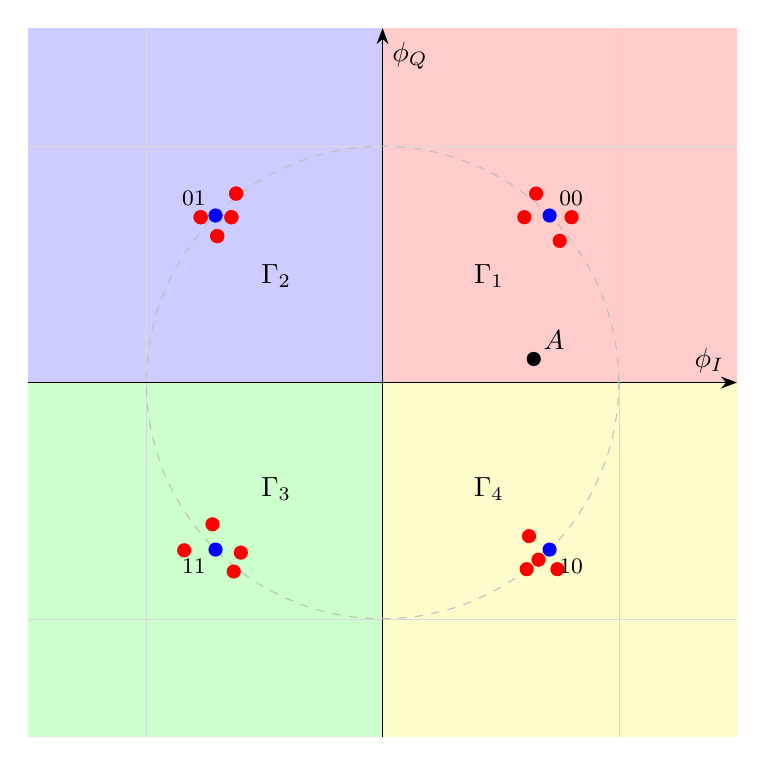
\begin{tikzpicture}[scale=3]

    % Fill the four quadrants with different colors
    \fill[red!20] (0,0) -- (1.5,0) -- (1.5,1.5) -- (0,1.5) -- cycle;
    \fill[blue!20] (0,0) -- (-1.5,0) -- (-1.5,1.5) -- (0,1.5) -- cycle;
    \fill[green!20] (0,0) -- (-1.5,0) -- (-1.5,-1.5) -- (0,-1.5) -- cycle;
    \fill[yellow!20] (0,0) -- (1.5,0) -- (1.5,-1.5) -- (0,-1.5) -- cycle;

    % Add region labels (Gamma)
    \node at (0.45,0.45) {$\Gamma_1$};
    \node at (-0.45,0.45) {$\Gamma_2$};
    \node at (-0.45,-0.45) {$\Gamma_3$};
    \node at (0.45,-0.45) {$\Gamma_4$};


    \draw[help lines,gray!30] (-1.5,-1.5) grid (1.5,1.5);
    
    \draw[-{Stealth[scale=1.2]}] (-1.5,0) -- (1.5,0) node[above, xshift=-10pt] {$\phi_I$};
    \draw[-{Stealth[scale=1.2]}] (0,-1.5) -- (0,1.5) node[right, yshift=-10pt] {$\phi_Q$};



    \draw[dashed,gray!50] (0,0) circle (1);

    % Received symbols
    \fill[red] (0.6,0.7) circle (0.03);
    \fill[red] (0.65,0.8) circle (0.03);
    \fill[red] (0.75,0.6) circle (0.03);
    \fill[red] (0.8,0.7) circle (0.03);

    \fill[red] (-0.6,-0.72) circle (0.03);
    \fill[red] (-0.63,-0.8) circle (0.03);
    \fill[red] (-0.72,-0.6) circle (0.03);
    \fill[red] (-0.84,-0.71) circle (0.03);

    \fill[red] (-0.64,0.7) circle (0.03);
    \fill[red] (-0.62,0.8) circle (0.03);
    \fill[red] (-0.7,0.62) circle (0.03);
    \fill[red] (-0.77,0.7) circle (0.03);

    \fill[red] (-0.64,0.7) circle (0.03);
    \fill[red] (-0.62,0.8) circle (0.03);
    \fill[red] (-0.7,0.62) circle (0.03);
    \fill[red] (-0.77,0.7) circle (0.03);

    \fill[red] (0.66,-0.75) circle (0.03);
    \fill[red] (0.61,-0.79) circle (0.03);
    \fill[red] (0.62,-0.65) circle (0.03);
    \fill[red] (0.74,-0.79) circle (0.03);
    
    % Some confusion points
    \fill[black] (0.64,0.1) circle (0.03);
    \node[above right] at (0.64,0.1) {$A$};
    
    % Constellation points
    \fill[blue] ({1/sqrt(2)},{1/sqrt(2)}) circle (0.03);
    \node[above right] at ({1/sqrt(2)},{1/sqrt(2)}) {\footnotesize 00};
    
    \fill[blue] ({-1/sqrt(2)},{1/sqrt(2)}) circle (0.03);
    \node[above left] at ({-1/sqrt(2)},{1/sqrt(2)}) {\footnotesize 01};
    
    \fill[blue] ({-1/sqrt(2)},{-1/sqrt(2)}) circle (0.03);
    \node[below left] at ({-1/sqrt(2)},{-1/sqrt(2)}) {\footnotesize 11};
    
    \fill[blue] ({1/sqrt(2)},{-1/sqrt(2)}) circle (0.03);
    \node[below right] at ({1/sqrt(2)},{-1/sqrt(2)}) {\footnotesize 10};
\end{tikzpicture}
\end{document}